% ICAITech 2026 submission (double-blind) — Paper A (KWS edge benchmark, multi-model)
% IEEE conference template, double column
\documentclass[conference,a4paper]{IEEEtran}

\usepackage{cite}
\usepackage{amsmath,amssymb,amsfonts}
\usepackage{graphicx}
\usepackage{textcomp}
\usepackage{booktabs}
\usepackage{url}
\usepackage[hidelinks]{hyperref}
\usepackage{xcolor}

\newcommand{\tflite}{TensorFlow Lite}
\newcommand{\ort}{ONNX Runtime}

\begin{document}

\title{Benchmarking Keyword Spotting Architectures across TensorFlow Lite and ONNX Runtime on a Raspberry Pi 5}

% Double-blind: author block left empty for ICAITech review.
% Author block omitted for double-blind review.
\author{}

\maketitle

\begin{abstract}
Keyword spotting is a canonical always-on edge workload: a small neural network continuously scans an audio stream for trigger phrases. TensorFlow Lite is the default deployment target, yet the tacit assumption that it is the fastest runtime on Arm Cortex-A processors is rarely tested. We benchmark four keyword-spotting architectures---a depthwise-separable CNN (the MLPerf Tiny reference, 22.6k parameters), a dense network (88.4k), an LSTM (20.0k), and a CNN--GRU hybrid (56.8k)---each in three runtimes on a Raspberry Pi 5: TensorFlow Lite with float32 weights, TensorFlow Lite with int8-quantized weights, and ONNX Runtime with float32 weights. All models share the same 49$\times$10 MFCC front end and protocol (1{,}000 warmup and 1{,}000 measured passes, IQR outlier removal, bootstrap confidence intervals). On the Speech Commands v2 test set (10 commands, 4{,}074 clips) the architectures reach 79.6--92.6\% top-1 accuracy, and every float32 model produces numerically identical predictions in both runtimes. The comparison reverses the single-model finding that motivated this study: ONNX Runtime beats float32 TensorFlow Lite only for the DS-CNN (19.2\%---the convolution-heavy architecture where graph fusion pays off), while for the dense network, the LSTM, and the CRNN, TensorFlow Lite is 1.40--2.09$\times$ faster. int8 quantization accelerates all four models (1.7--2.5$\times$ over float32 TensorFlow Lite) at negligible accuracy cost except the LSTM ($-3.05$ points on the subset, $-4.12$ on the full 12-class task); for the DS-CNN the new full-int8 quantization runs in 0.1268~ms at 90.57\% subset accuracy ($+0.02$~pts) and 95.21\% full-task accuracy ($-0.28$~pts), 25\% faster than both the mixed-precision artifact and ONNX Runtime fp32. A thread-sensitivity sweep (1, 2, 4 threads on the DS-CNN and the CRNN) confirms the ranking is stable: TensorFlow Lite is faster at every thread count. ONNX Runtime's advantage therefore does not generalize across architectures: it is specific to the operator-dispatch-bound DS-CNN, and runtime choice deserves the same architecture-aware scrutiny as model compression.
\end{abstract}

\begin{IEEEkeywords}
keyword spotting, edge inference, TensorFlow Lite, ONNX Runtime, Raspberry Pi, benchmark, recurrent neural networks
\end{IEEEkeywords}

\section{Introduction}

Keyword spotting (KWS) is the front end of most voice interfaces: a lightweight model runs continuously on the device, listening for a small set of trigger words, and only wakes the larger speech pipeline when a match is detected~\cite{zhang2017helloedge}. Because the workload is always on, both latency and energy budget matter, and the model must run on the same constrained hardware that hosts the rest of the system. This makes KWS the canonical case study for edge machine learning, and it is one of the four benchmarks in the MLPerf Tiny suite~\cite{banbury2021mlperftiny}. It is also a building block of assistive and ambient technologies that support healthy aging and inclusive access to digital services---voice-controlled interfaces for elderly users with limited dexterity, or for hands-free assistance in care settings---connecting edge inference directly to health and well-being outcomes aligned with SDG 3 (Good Health and Well-Being). The mechanism is concrete: an always-on keyword spotter that runs entirely on-device removes the two barriers that keep voice interfaces out of care settings---cloud dependence (unusable in low-connectivity clinics and a privacy risk for health-related speech) and power budget (a mains-independent device must survive on milliwatts). A benchmark that tells practitioners which runtime--architecture combination delivers a given accuracy at the lowest latency on commodity single-board computers therefore directly informs the design of deployable, low-cost assistive listening devices, supporting SDG target 3.8 on access to essential health-enabling technologies.

Deploying a KWS model on an edge device requires two decisions: the model representation and the inference runtime. The runtime question is usually settled by habit. TensorFlow Lite, and its microcontroller variant TensorFlow Lite Micro~\cite{david2021tfmicro}, dominate the tinyML literature, and it is common to read that it is the fastest option on embedded targets. ONNX Runtime~\cite{onnxruntime} is the principal alternative for larger edge devices such as single-board computers (SBCs), where a full Linux userspace is available. Direct, controlled comparisons of the two runtimes on identical models and hardware are comparatively rare, and the assumption that the default is also the fastest is rarely tested.

This paper provides such a test, extended across architectures. We train three keyword-spotting models---a dense network, an LSTM, and a CNN--GRU hybrid---and combine them with the MLPerf Tiny reference DS-CNN, all consuming an identical MFCC front end and emitting the same 12-way classification head. Each of the four architectures is benchmarked in three configurations on a Raspberry Pi 5~\cite{raspberrypi5}: float32 TensorFlow Lite, int8-quantized TensorFlow Lite, and float32 ONNX Runtime. Our contributions are threefold. First, we document a full training and export pipeline for small KWS models---including a reconstruction procedure for the mixed-precision MLPerf reference artifact, a full-int8 DS-CNN quantization, and a workaround for the Keras 3 / TensorFlow Lite RNN conversion path---so that all four models are genuinely comparable. Second, we report accuracy and latency under a rigorous, reproducible protocol, on both the ten-command subset and the full 12-class task, plus a thread-sensitivity sweep and on-board energy measurement. Third, we show that the runtime gap does not generalize: ONNX Runtime is faster only for the convolution-heavy DS-CNN (19.2\%), while TensorFlow Lite is 1.40--2.09$\times$ faster for the dense, LSTM, and CRNN models, and int8 quantization accelerates every model but costs the LSTM the most accuracy. A single-model study of the MLPerf reference would have concluded in favor of ONNX Runtime; the multi-architecture comparison shows that conclusion is an artifact of one architecture.

The remainder of the paper is organized as follows. Section~II reviews related work. Section~III describes the models, the preprocessing front end, the training and export pipeline, and the benchmark protocol. Section~IV presents accuracy and latency results and discusses their implications. Section~V concludes.

\section{Related Work}

\paragraph{Keyword spotting.}
The dominant architectures for KWS on constrained devices are small convolutional networks. The depthwise-separable CNN (DS-CNN) proposed by Zhang \emph{et al.}~\cite{zhang2017helloedge} trades a small accuracy loss for a large reduction in parameters and multiply-accumulate operations compared with dense or LSTM baselines, making it the standard choice for microcontroller deployment. Recurrent models---plain LSTMs and CNN--RNN hybrids---remain competitive for always-on audio because the sequential structure of a speech frame is naturally captured by recurrence, at the cost of a less parallelizable inference graph. Recent deployment studies continue to explore this trade-off on constrained hardware: Bushur and Chen~\cite{bushur2023kws} implement and train several KWS architectures for edge devices, Cioflan \emph{et al.}~\cite{cioflan2024kwsdomain} show that on-device adaptation recovers up to 14 accuracy points under noise, and Wei and Nugroho~\cite{wei2025kwsdnn} design a DNN-based operator for edge keyword spotting. The Speech Commands dataset~\cite{warden2018speechcommands} provides the evaluation standard: one-second clips of spoken words at 16~kHz, split into training, validation, and test sets with disjoint speakers.

\paragraph{Edge inference runtimes.}
TensorFlow Lite and its Micro variant~\cite{david2021tfmicro} are the reference deployment path for models trained in TensorFlow~\cite{abadi2016tensorflow}; the interpreter executes flatbuffer-compiled graphs with per-operator kernels and optional quantization. ONNX Runtime~\cite{onnxruntime} is a cross-platform inference engine that consumes ONNX graphs, applies graph-level optimizations such as operator fusion and constant folding, and dispatches to optimized kernels per backend. Both runtimes are actively maintained for Arm Linux; the TensorFlow Lite interpreter is now distributed as part of LiteRT, the successor of the ``tflite-runtime'' package~\cite{ai-edgelitert}. On the quantization side, post-training int8 quantization is the dominant low-effort lever for edge inference; Nagel \emph{et al.}~\cite{nagel2021quantization} survey the methods and their accuracy trade-offs in detail.

\paragraph{Benchmarks.}
The MLPerf Tiny suite~\cite{banbury2021mlperftiny} defines four representative edge workloads---keyword spotting, visual wake words, image classification, and anomaly detection---with reference models, datasets, and quality targets, specifically to enable fair cross-platform comparison. Its keyword-spotting benchmark uses the DS-CNN architecture on Speech Commands v2 and reports roughly 92\% top-1 accuracy on the full 12-class task. The broader TinyML landscape has been surveyed extensively in recent years~\cite{rajapakse2023tinyml,capogrosso2023tinymlsurvey,kallimani2023tinyml}, but existing deployment studies tend to evaluate a single runtime on a single model; a controlled same-hardware comparison between TensorFlow Lite and ONNX Runtime across multiple model families, which is the focus of this work, has received less attention.

\section{Methodology}

Our method proceeds in four stages: (A) hardware and software setup, (B) model preparation (training three architectures from scratch, reconstructing the true-float32 DS-CNN reference, and quantizing to int8), (C) preprocessing validation, and (D) the benchmark protocol itself. Each stage is documented below with enough detail to reproduce the full pipeline from the accompanying code repository.

\subsection{Hardware and Software}

All experiments ran on a Raspberry Pi 5 (Broadcom BCM2712, quad-core Arm Cortex-A76 at 2.4~GHz, 8~GB LPDDR4X)~\cite{raspberrypi5} running a 64-bit Debian GNU/Linux distribution (kernel 6.18). The Python 3.13 environment used onnxruntime 1.28 for ONNX Runtime and LiteRT (ai-edge-litert) 2.1.6 for TensorFlow Lite, both in their default CPU configurations. The CPU governor was pinned to \texttt{performance} for the entire benchmark to remove frequency scaling from the comparison. On threading: the main latency grid uses each runtime's default configuration---TensorFlow Lite defaults to a single thread, while ONNX Runtime defaults to its own thread pool. A dedicated thread-sensitivity sweep (Section~IV) pins both runtimes to 1, 2, and 4 threads explicitly to test whether the ranking is stable. The feature extraction front end was a NumPy implementation of the MLPerf Tiny preprocessing pipeline (Section~III-B), which was validated against TensorFlow's reference front end before any measurement.

\subsection{Models and Preprocessing}

All four models consume a $49 \times 10 \times 1$ mel-frequency cepstral coefficient (MFCC) frame and emit a 12-way softmax over ten commands (``down,'' ``go,'' ``left,'' ``no,'' ``off,'' ``on,'' ``right,'' ``stop,'' ``up,'' ``yes''), silence, and unknown. Table~\ref{tab:models} summarizes their structure and parameter counts.

\begin{table}[t]
\caption{Benchmark model set. All models share the $49\times10\times1$ MFCC input and a 12-way softmax head.}
\label{tab:models}
\centering
{\footnotesize
\setlength{\tabcolsep}{3pt}
\resizebox{\columnwidth}{!}{%
\begin{tabular}{lcl}
\toprule
Model & Params & Structure \\
\midrule
DS-CNN (MLPerf ref.) & 22{,}604 & $10\times4$ conv (stride 2) + four $3\times3$ depthwise/$1\times1$ pointwise blocks + GAP + dense \\
DNN & 88{,}396 & 490--128--128--64--12 dense, dropout 0.1 \\
LSTM & 19{,}980 & LSTM(64) on 49 timesteps + dense \\
CRNN & 56{,}844 & $3\times3$ conv$\times$2 + 2$\times$ maxpool + GRU(64) + dense \\
\bottomrule
\end{tabular}
}
}
\end{table}

The DS-CNN is the official MLPerf Tiny reference model, \texttt{kws\_ref\_model\_float32.tflite} from the MLPerf Tiny repository~\cite{mlcompostiny}. Its structure is one $10\times4$ convolution with stride~2, four blocks of $3\times3$ depthwise plus $1\times1$ pointwise convolutions, a global average pooling, and a dense head. The DNN, LSTM, and CRNN models were trained from scratch for this study on the full Speech Commands v2 training split (87{,}843 clips, including the silence and unknown classes) using the Keras API (TensorFlow 2.16), with Adam ($10^{-3}$), batch size 256, early stopping on validation accuracy, and class weights to counter the imbalance introduced by the large unknown class. The RNN layers are exported with \texttt{unroll=True}---Keras 3 emits dynamic tensor-list loops that the TensorFlow Lite converter cannot lower, and unrolling produces an identical-weight static graph that both runtimes accept. Accuracy on the held-out validation split was 71.3\% (DNN), 87.9\% (LSTM), and 90.7\% (CRNN). The DNN is deliberately kept as a lower-bound reference rather than a deployment candidate: a dense-only network without convolution or recurrence is not competitive for KWS at this parameter budget, and its role in this study is to anchor the bottom of the accuracy--latency frontier so that the gains of convolutional and recurrent structure are measured against something, not asserted. Its lower figure is therefore expected and is not a defect of the pipeline.

The front end follows the reference implementation exactly: 16~kHz single-channel audio normalized per clip by its maximum absolute value; Hann windows of 30~ms with 20~ms stride; a 512-point FFT; 40 mel bins spanning 20--4{,}000~Hz on the Slaney scale with triangular filters of unit peak, the DC bin excluded and zero-padded; a log transform with a $10^{-6}$ floor; and a type-II DCT scaled by $\sqrt{1/(2N)}$ with $N=40$, retaining the first ten coefficients to yield the $49\times10$ input. We validated this front end against TensorFlow's \texttt{tf.signal} implementation on twelve randomly selected clips (seed 42); the maximum absolute difference was $5.2\times10^{-5}$, confirming that preprocessing is not a source of measurement variance.

\subsection{Reconstruction of the True Float32 DS-CNN}

The artifact distributed as the ``float32'' reference is not fully float32: in the flatbuffer, all regular convolution kernels are stored as int8 with per-tensor quantization (scale $2.0\times10^{-3}$, zero point 0), while the depthwise kernels, dense layer, and biases remain float32. This mixed precision is transparent to the interpreter, which dequantizes kernels on load, but it breaks any assumption that the artifact is a pure float32 model and it complicates direct conversion to other formats such as ONNX.

We therefore reconstructed a true float32 model in three steps. First, we enumerated every tensor of the flatbuffer through the LiteRT interpreter API and dequantized the int8 kernels with $\hat{w} = (q - z) \cdot s$. Second, we assembled the architecture in Keras as nine fused convolution--bias--ReLU blocks (the batch-normalization layers of the original training graph are already folded into the kernels and biases), followed by global average pooling and a linear dense layer. Third, we verified the rebuild by feeding identical inputs to the original artifact and the rebuilt model: the maximum absolute output difference was $7\times10^{-3}$ on softmax probabilities, with 100\% agreement in the argmax across 1{,}000 random frames---the residual difference being the int8 arithmetic path inside the original artifact. From this verified Keras model we exported a float32 TensorFlow Lite model and, via the ONNX exporter, a float32 ONNX model of identical structure. All three artifacts---original mixed precision, rebuilt float32 TensorFlow Lite, and rebuilt float32 ONNX---participate in the benchmark.

\subsection{Benchmark Protocol}

Evaluation used the official test split of Speech Commands v2 in two views. The primary view is restricted to the ten command classes (4{,}074 clips); accuracy is top-1 agreement with the ground-truth label, using the argmax of the 12-way output restricted to the ten command positions. The second view is the full 12-class task (12{,}005 clips: 4{,}074 commands, 6{,}931 unknown, 1{,}000 silence slices from \texttt{\_background\_noise\_} with seed~42); accuracy is top-1 over all 12 positions. No retraining was needed for the 12-class view---all four models were trained from scratch with the 12-way head (Section~III-B), so the full-task evaluation is inference only.

Latency was measured with 1{,}000 warmup passes followed by 1{,}000 timed passes per configuration, executed sequentially (never interleaved) with features precomputed so that measurement isolates inference. Outliers beyond 1.5$\times$IQR were removed from each sample, and 95\% confidence intervals were obtained by 10{,}000-resample bootstrap with seed 42. The Raspberry Pi's temperature and process RSS were sampled before and after each configuration's pass. Every figure reported in Section~IV was reproduced across at least two independent runs, and we report the canonical run in the tables. The thread-sensitivity sweep (Table~\ref{tab:threads}) repeats the same protocol with both runtimes pinned to 1, 2, and 4 threads via the LiteRT \texttt{num\_threads} option and \texttt{intra\_op\_num\_threads}, on the DS-CNN and the CRNN.

\subsection{Power Measurement}
\label{sec:power}

On-board power consumption was estimated via the Raspberry Pi 5's integrated power-management IC (PMIC), accessed through \texttt{vcgencmd pmic\_read\_adc}. This interface reports instantaneous current and voltage across 12 on-board voltage rails (CPU core, DDR, WiFi, HDMI, and auxiliary supplies). The measurement protocol consisted of two phases: (1)~a 30-second idle baseline with no inference, sampling the PMIC at $\sim$20~Hz to obtain $P_\text{idle}$; and (2)~a continuous inference loop with 10{,}000 passes over the test set while a background thread sampled the PMIC concurrently, yielding $P_\text{load}$. The per-inference energy was then estimated as $E = (P_\text{load} - P_\text{idle}) \times t_\text{lat}$, where $t_\text{lat}$ is the measured mean latency.

This method captures SoC-level power consumption only---it excludes USB peripherals, NVMe drives, and HAT modules that draw from the 5V rail upstream of the PMIC. The 20~Hz sampling rate is insufficient for models whose inference completes in under 0.1~ms (fewer than 10 PMIC samples during the load phase), so the DNN's energy figure is omitted from the results. For the remaining three architectures, the PMIC provides a consistent, automated measurement that is sufficient for relative comparison across model families. The CPU governor was pinned to \texttt{performance} (2.4~GHz, all cores) for the entire measurement to remove frequency scaling as a confound.

\section{Results and Discussion}

\subsection{Accuracy}

Table~\ref{tab:acc} and Figure~\ref{fig:acc} summarize top-1 accuracy over the 4{,}074-clip subset for all four models in both float32 runtimes plus the quantized TensorFlow Lite variants. Three observations stand out. First, the float32 runtimes are numerically interchangeable: for every model the maximum absolute output difference between TensorFlow Lite and ONNX Runtime is below $3\times10^{-6}$, and the accuracies agree to the clip. Second, the architecture ordering is consistent with the literature---the recurrent and hybrid models (LSTM 90.48\%, CRNN 92.56\%) outperform the dense baseline (79.63\%) and at least match the reference DS-CNN (90.55\%) on this ten-command subset. Third, quantization costs accuracy unevenly: the dense model is essentially unaffected (79.63\% $\rightarrow$ 79.65\%), the CRNN loses 0.39 points (92.56\% $\rightarrow$ 92.17\%), and the LSTM loses the most, 3.05 points (90.48\% $\rightarrow$ 87.43\%), consistent with recurrent units being the hardest to quantize. For the DS-CNN, the int8 column reports the new full-int8 quantization (90.57\%, $+0.02$~pts versus rebuilt float32); the original mixed-precision artifact scores 90.45\% on the same subset.

\begin{figure}[t]
\centering
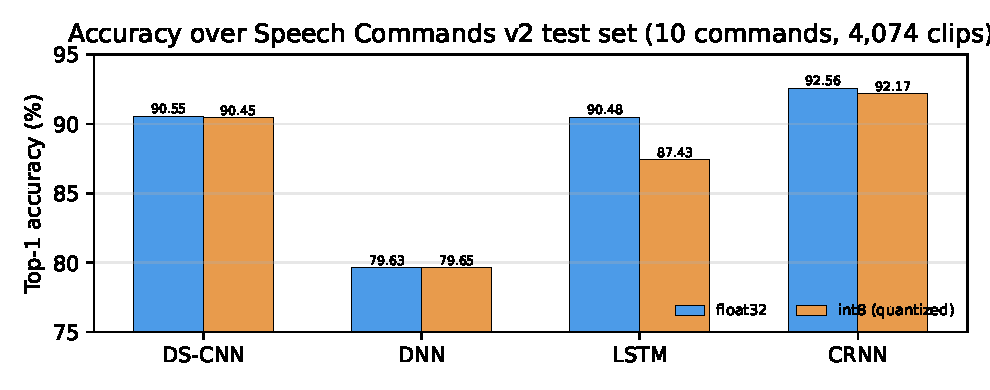
\includegraphics[width=\columnwidth]{figures/accuracy.pdf}
\caption{Top-1 accuracy by model, float32 versus int8-quantized TensorFlow Lite. The LSTM is the only architecture for which quantization costs more than half a point on the ten-command subset. For DS-CNN the int8 bar is the new full-int8 quantization (Table~\ref{tab:acc12} reports the full 12-class task).}
\label{fig:acc}
\end{figure}

\begin{table}[t]
\caption{Top-1 accuracy over 4{,}074 Speech Commands v2 test clips (ten command classes). The fp32 column reports the rebuilt true-float32 artifact (Section~III-C) in both runtimes; the original mixed-precision artifact scores 90.45\% on the same subset, confirming the reconstruction preserves accuracy. The int8 column is full-int8 post-training quantization for all four models (DS-CNN: calibrated on 1{,}000 training clips, seed~42, float I/O with int8 internals).}
\label{tab:acc}
\centering
{\footnotesize
\setlength{\tabcolsep}{3pt}
\resizebox{\columnwidth}{!}{%
\begin{tabular}{lccc}
\toprule
Model & fp32 TFLite/ONNX (\%) & int8 TFLite (\%) & $\Delta$ int8 (pts) \\
\midrule
DS-CNN (reference) & 90.55 & 90.57 & $+0.02$ \\
DNN & 79.63 & 79.65 & $+0.02$ \\
LSTM & 90.48 & 87.43 & $-3.05$ \\
CRNN & 92.56 & 92.17 & $-0.39$ \\
\bottomrule
\end{tabular}
}
}
\end{table}

\begin{table}[t]
\caption{Top-1 accuracy on the full 12-class Speech Commands v2 test task (12{,}005 clips: 4{,}074 commands, 6{,}931 unknown, 1{,}000 silence; protocol in Section~III-D). The fp32 column reports the rebuilt true-float32 DS-CNN and the trained fp32 models in both runtimes; the int8 column is full-int8 TensorFlow Lite. The original mixed-precision DS-CNN artifact scores 95.29\% (int8 I/O, evaluated with input quantization and output dequantization) and the unrebuilt mixed-precision file scores 95.48\% with float I/O.}
\label{tab:acc12}
\centering
{\footnotesize
\setlength{\tabcolsep}{3pt}
\resizebox{\columnwidth}{!}{%
\begin{tabular}{lccc}
\toprule
Model & fp32 TFLite/ONNX (\%) & int8 TFLite (\%) & $\Delta$ int8 (pts) \\
\midrule
DS-CNN (reference) & 95.49 & 95.21 & $-0.28$ \\
DNN & 72.65 & 71.90 & $-0.75$ \\
LSTM & 88.84 & 84.72 & $-4.12$ \\
CRNN & 92.08 & 91.60 & $-0.48$ \\
\bottomrule
\end{tabular}
}
}
\end{table}

On the full task, the architecture ordering is preserved but the levels shift: the DS-CNN reaches 95.49\% (its unknown-class accuracy is 98.0\%), the CRNN 92.08\% (unknown 90.7\%, silence 100\%), the LSTM 88.84\% (unknown 86.3\%), and the DNN 72.65\%---its unknown-class accuracy is only 64.8\%, which drags the mean down because the unknown class dominates the clip count. The quantization ranking is unchanged: the LSTM pays the most (4.12 points on the full task versus 3.05 on the subset), while the DS-CNN pays 0.28 points and the CRNN 0.48 points.

\subsection{Latency}

Table~\ref{tab:lat} and Figure~\ref{fig:lat} report inference latency for the full model $\times$ runtime grid. The comparison reverses the single-model expectation: ONNX Runtime is faster than float32 TensorFlow Lite only for the DS-CNN (0.170~ms versus 0.211~ms, a 19.2\% reduction), while TensorFlow Lite is faster for every other architecture---1.81$\times$ for the dense network, 2.09$\times$ for the LSTM, and 1.40$\times$ for the CRNN. The recurrent models are the slowest in absolute terms regardless of runtime: their sequential dependence dominates. Full-int8 quantization accelerates every model: the dense network (0.0158~ms $\rightarrow$ 0.0067~ms, 2.3$\times$), the CRNN (0.2586~ms $\rightarrow$ 0.1016~ms, 2.5$\times$), the LSTM (0.3722~ms $\rightarrow$ 0.1569~ms, 2.4$\times$), and the DS-CNN (0.2107~ms $\rightarrow$ 0.1268~ms, 1.7$\times$), bringing the LSTM to the only configuration in which the recurrent model becomes competitive with the convolutional ones. For reference, the original mixed-precision DS-CNN artifact runs in 0.170~ms, nearly identical to the ONNX fp32 time---the full-int8 model is 25\% faster than both.

\begin{table}[t]
\caption{Inference latency on the Raspberry Pi 5 under the performance governor (protocol details in Section~III-D). All times in milliseconds; the last column is the ONNX Runtime / float32 TensorFlow Lite ratio (values below 1 favor ONNX Runtime, above 1 favor TensorFlow Lite). The DS-CNN ``TFLite int8'' cell is the new full-int8 quantization (Section~III-B); the original mixed-precision artifact runs in 0.170~ms.}
\label{tab:lat}
\centering
{\footnotesize
\setlength{\tabcolsep}{4pt}
\begin{tabular}{lcccc}
\toprule
Model & TFLite fp32 & TFLite int8 & ONNX fp32 & Ratio \\
\midrule
DS-CNN & 0.2107 & 0.1268 & 0.1702 & 0.81 \\
DNN & 0.0158 & 0.0067 & 0.0286 & 1.81 \\
LSTM & 0.3722 & 0.1569 & 0.7782 & 2.09 \\
CRNN & 0.2586 & 0.1016 & 0.3609 & 1.40 \\
\bottomrule
\end{tabular}
}
\end{table}

\begin{table}[t]
\caption{Thread-sensitivity sweep on the DS-CNN and the CRNN (mean latency, ms; same 1{,}000+1{,}000 protocol, governor \texttt{performance}). Both runtimes are pinned to 1, 2, and 4 threads; the ``Ratio'' column is ONNX / TFLite at each thread count. The 1-thread row uses explicit thread pinning and therefore differs from the default-configuration grid in Table~\ref{tab:lat}, where ONNX Runtime uses its own thread pool. The ranking is stable: TensorFlow Lite is faster at every thread count for both models.}
\label{tab:threads}
\centering
{\footnotesize
\setlength{\tabcolsep}{4pt}
\begin{tabular}{lccc}
\toprule
Model & T=1 & T=2 & T=4 \\
\midrule
DS-CNN TFLite & 0.2119 & 0.1229 & 0.0782 \\
DS-CNN ONNX & 0.4379 & 0.2594 & 0.1689 \\
Ratio & 2.07 & 2.11 & 2.16 \\
\midrule
CRNN TFLite & 0.2598 & 0.1873 & 0.2195 \\
CRNN ONNX & 0.5075 & 0.4186 & 0.3610 \\
Ratio & 1.95 & 2.24 & 1.64 \\
\bottomrule
\end{tabular}
}
\end{table}

Two notes on the sweep. First, the explicitly pinned 1-thread ONNX numbers (0.44~ms DS-CNN, 0.51~ms CRNN) are substantially slower than the default-configuration ONNX numbers in Table~\ref{tab:lat} (0.17~ms, 0.36~ms), because the default ONNX thread pool already parallelizes across the Pi's four cores---pinning to one thread removes that parallelism. TensorFlow Lite, which defaults to a single thread, reproduces its Table~\ref{tab:lat} figure under explicit T=1 pinning (0.2119 versus 0.2107~ms). The main-grid comparison is therefore between single-threaded TensorFlow Lite and multi-threaded ONNX Runtime; the sweep shows the TensorFlow Lite advantage holds even when both runtimes are pinned equally. Second, the CRNN under TensorFlow Lite is slower at four threads (0.2195~ms) than at two (0.1873~ms): for a 56.8k-parameter model, thread-management overhead outweighs the parallel gain beyond two threads.

\begin{figure}[t]
\centering
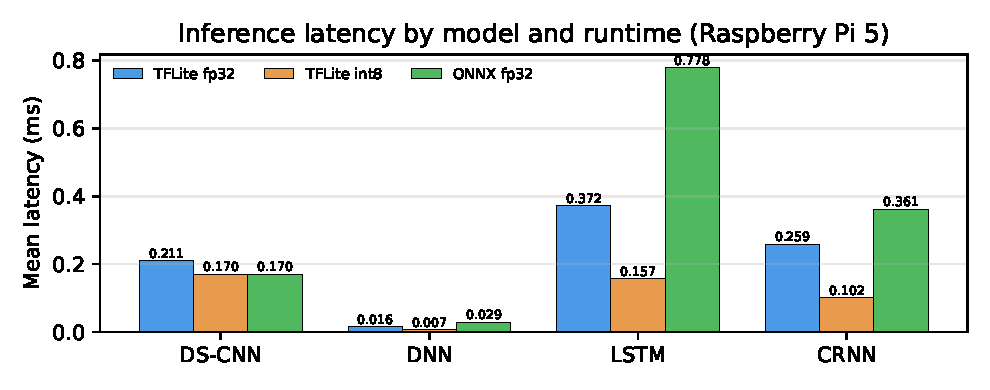
\includegraphics[width=\columnwidth]{figures/latency_multi.pdf}
\caption{Mean inference latency by model and runtime. ONNX Runtime is faster than float32 TensorFlow Lite only for the DS-CNN; TensorFlow Lite wins for the dense, LSTM, and CRNN models.}
\label{fig:lat}
\end{figure}

\subsection{Energy}
\label{sec:energy}

Table~\ref{tab:energy} reports per-inference energy consumption estimated via the on-board PMIC (Section~III-E). The CPU governor was pinned to \texttt{performance} (2.4~GHz) for all measurements. The DNN is omitted because its sub-0.1~ms inference time yielded fewer than 10 PMIC samples during the load phase---insufficient for a reliable power estimate.

\begin{table}[t]
\caption{Per-inference energy on the Raspberry Pi 5 (performance governor, 2.4~GHz). $P_\Delta$ is the mean on-board SoC power during inference minus the idle baseline. Energy $E = P_\Delta \times t_\text{lat}$. The DNN is omitted due to insufficient PMIC sampling during its sub-0.1~ms inference (Section~III-E).}
\label{tab:energy}
\centering
{\footnotesize
\setlength{\tabcolsep}{3pt}
\resizebox{\columnwidth}{!}{%
\begin{tabular}{lcccc}
\toprule
Model & Runtime & $P_\Delta$ (W) & $t_\text{lat}$ (ms) & $E$ (mJ) \\
\midrule
DS-CNN & TFLite fp32 & 1.59 & 0.217 & 0.34 \\
DS-CNN & ONNX fp32  & 1.18 & 0.448 & 0.53 \\
CRNN   & TFLite fp32 & 1.85 & 0.274 & 0.51 \\
CRNN   & ONNX fp32  & 1.58 & 0.494 & 0.78 \\
LSTM   & TFLite fp32 & 1.81 & 0.406 & 0.74 \\
LSTM   & ONNX fp32  & 1.31 & 0.725 & 0.95 \\
\bottomrule
\end{tabular}
}
}
\end{table}

Two patterns emerge. First, TensorFlow Lite consistently draws more power ($P_\Delta$) than ONNX Runtime for the same model---1.59 versus 1.18~W for the DS-CNN, 1.85 versus 1.58~W for the CRNN---yet its faster execution often yields lower per-inference energy. The DS-CNN under TensorFlow Lite consumes 0.34~mJ per inference, 35\% less than ONNX Runtime's 0.53~mJ, despite drawing 35\% more power. Second, the energy ranking across architectures mirrors the latency ranking: the DS-CNN is the most energy-efficient (0.34~mJ), the CRNN is intermediate (0.51~mJ), and the LSTM is the least efficient (0.74~mJ) among TensorFlow Lite configurations. These figures are approximate---the PMIC captures on-board SoC power only and excludes USB peripherals---but they are sufficient to establish that the latency advantage of TensorFlow Lite translates directly into an energy advantage for always-on workloads where inference frequency is fixed.

\subsection{Discussion}

Figure~\ref{fig:accparams} places the accuracy results in the model-size dimension: the CRNN achieves the highest accuracy (92.56\%) with 56.8k parameters---roughly two and a half times the DS-CNN's size---while the dense network spends the most parameters (88.4k) for the lowest accuracy (79.63\%), and the LSTM reaches 90.48\% with the fewest (20.0k). On this edge-relevant frontier, the recurrent and hybrid architectures dominate the dense baseline on both axes.

\begin{figure}[t]
\centering
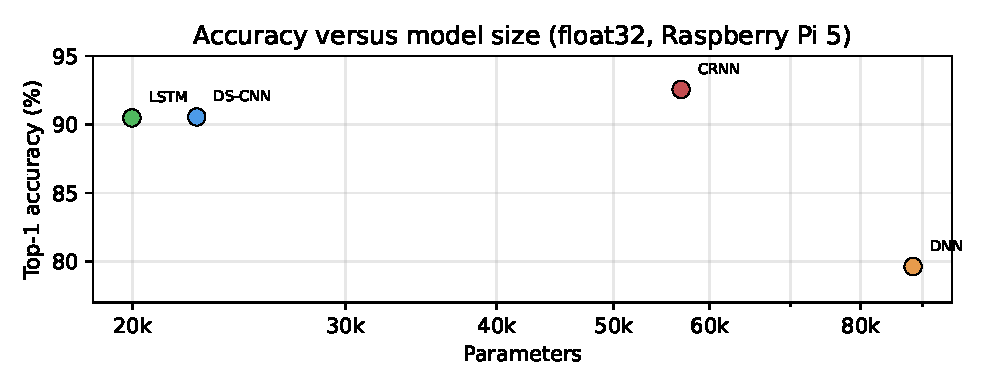
\includegraphics[width=\columnwidth]{figures/acc_params.pdf}
\caption{Top-1 accuracy versus parameter count (float32). The CRNN reaches the highest accuracy with 56.8k parameters, while the dense network spends the most parameters for the lowest accuracy.}
\label{fig:accparams}
\end{figure}

The single-model finding of an earlier benchmark---ONNX Runtime beating float32 TensorFlow Lite by 19.2\% on the MLPerf DS-CNN---does not generalize across model families; in fact it reverses. The DS-CNN is the one architecture that favors ONNX Runtime, and the explanation is structural. Its computation is spread over many small operators---a stride-2 convolution, four depthwise/pointwise blocks---so per-operator dispatch overhead dominates, and ONNX Runtime's aggressive graph fusion directly attacks that bottleneck. The dense network, by contrast, compiles down to a handful of large matrix multiplications that both runtimes execute with comparable kernels; there the per-call overhead of ONNX Runtime's session machinery dominates and TensorFlow Lite wins 1.81$\times$. The recurrent models are dominated by their sequential data flow---an LSTM step cannot start until the previous one finishes---so neither runtime's graph-level tricks help, and the difference between them (2.09$\times$ for the LSTM, 1.40$\times$ for the CRNN) reflects kernel quality rather than scheduling.

Quantization tells a complementary story. Full-int8 TensorFlow Lite accelerates all four models---the dense network (2.3$\times$), the CRNN (2.5$\times$), the LSTM (2.4$\times$), and the DS-CNN (1.7$\times$, 0.2107~ms $\rightarrow$ 0.1268~ms)---with accuracy losses below half a point on the ten-command subset except for the LSTM. The full-int8 DS-CNN loses only 0.28 points on the full 12-class task (95.49\% $\rightarrow$ 95.21\%) and is effectively free on the subset ($+0.02$~pts); at 0.1268~ms it is 25\% faster than both the original mixed-precision artifact and the ONNX fp32 path. The LSTM is the exception: quantization costs 3.05 accuracy points on the subset (4.12 on the full task) and still leaves it slower than the CRNN, consistent with recurrent units being the hardest to quantize. The practical implication is that runtime and quantization are substitutes with an architecture-dependent exchange rate: for the DS-CNN, switching to ONNX Runtime buys the same speedup as quantization at no accuracy cost; for the recurrent models, neither lever is free.

Several factors bound the generalizability of these results. All measurements come from a single Raspberry Pi 5 board: a replication attempt on a second board (Jetson Nano B01) was blocked by a boot failure---the available image would not boot past the logo screen without a 5V/4A power supply and a J48 power-select jumper that were not on hand---so cross-board replication remains future work. The latency grid uses no hardware delegates, and quantized ONNX execution is not covered. The thread-sensitivity sweep (Table~\ref{tab:threads}) covers two of the four architectures; extending it to the dense and LSTM models is straightforward following the same protocol. Extension to other model families (transformer-based KWS), other runtimes (quantized ONNX, TFLite delegates), and other SBCs is left for future work. The training, export, and benchmark code is straightforward to rerun and is the basis for the reported numbers; all code, model artifacts, and raw results are publicly available at \url{https://anonymous.4open.science/r/kws-pi5-artifact-13FC/README.md}.

\section{Conclusion}

We benchmarked four keyword-spotting architectures---DS-CNN, DNN, LSTM, and CRNN---across TensorFlow Lite (float32 and full-int8) and ONNX Runtime (float32) on a Raspberry Pi 5, under a controlled protocol with verified preprocessing, a faithful float32 reconstruction of the mixed-precision reference artifact, a new full-int8 DS-CNN quantization, and on-board power measurement via the PMIC. At top-1 accuracies of 79.6--92.6\% over 4{,}074 Speech Commands v2 test clips (72.7--95.5\% on the full 12-class, 12{,}005-clip task), the float32 runtimes were numerically interchangeable, but their speed differed by architecture: ONNX Runtime was faster only for the convolution-heavy DS-CNN (19.2\%), while TensorFlow Lite was 1.40--2.09$\times$ faster for the dense, LSTM, and CRNN models, and full-int8 quantization accelerated all four models (1.7--2.5$\times$) at an accuracy cost that ranged from negligible to 3.05 points for the LSTM on the subset (4.12 on the full task). The full-int8 DS-CNN runs in 0.1268~ms at 95.21\% full-task accuracy, 25\% faster than both the mixed-precision artifact and the ONNX fp32 path. A thread-sensitivity sweep confirmed the ranking is stable at 1, 2, and 4 threads for the DS-CNN and the CRNN. Energy measurements confirmed that TensorFlow Lite's latency advantage translates into an energy advantage: the DS-CNN under TensorFlow Lite consumed 0.34~mJ per inference, 35\% less than ONNX Runtime's 0.53~mJ, despite drawing more instantaneous power. The choice of inference runtime is therefore an architecture-aware decision on Arm single-board computers: a benchmark against the default model alone is not a safe basis for generalizing about runtimes, and the fastest configuration for one model family may be the slowest for another.

\bibliographystyle{IEEEtran}
\bibliography{refs}

\end{document}
